% ============================================================================
% NAS-YOLO: Noise-Aware State Modeling for Robust Real-Time Object Detection
% ECCV 2026 Submission
% ============================================================================
\documentclass[review]{eccv2026}

\usepackage{cite}
\usepackage{bm}
\usepackage{pifont}
\usepackage{colortbl}

% Custom commands
\newcommand{\ours}{\textbf{NAS-YOLO}}
\newcommand{\ie}{\textit{i.e.}}
\newcommand{\eg}{\textit{e.g.}}
\newcommand{\cf}{\textit{cf.}}
\newcommand{\etal}{\textit{et al.}}
\newcommand{\wrt}{w.r.t.}
\newcommand{\cmark}{\ding{51}}
\newcommand{\xmark}{\ding{55}}
\newcommand{\bsi}{\text{BSI}}
\newcommand{\mapc}{\text{mAP-C}}
\newcommand{\R}{\mathbb{R}}

% Color for table highlights
\definecolor{bestcolor}{RGB}{200,230,200}
\definecolor{secondcolor}{RGB}{220,240,255}
\newcommand{\best}[1]{\textbf{#1}}
\newcommand{\second}[1]{\underline{#1}}

% ============================================================================
% RESULT PLACEHOLDERS -- Update this block when experiments complete.
% All table cells and in-text claims reference these macros.
% ============================================================================
% --- NAS-YOLO-n results ---
\newcommand{\nasNmap}{XX.X}
\newcommand{\nasNmapFifty}{XX.X}
\newcommand{\nasNmapC}{XX.X}
\newcommand{\nasNbsi}{X.XXX}
\newcommand{\nasNfps}{XXX}
% --- NAS-YOLO-s results ---
\newcommand{\nasSmap}{XX.X}
\newcommand{\nasSmapFifty}{XX.X}
\newcommand{\nasSmapC}{XX.X}
\newcommand{\nasSbsi}{X.XXX}
\newcommand{\nasSfps}{XXX}
% --- Baseline mAP-C (to be measured) ---
\newcommand{\yoloEightNmapC}{XX.X}
\newcommand{\yoloEightNbsi}{X.XXX}
\newcommand{\yoloNineTmapC}{XX.X}
\newcommand{\yoloNineTbsi}{X.XXX}
\newcommand{\yoloTenNmapC}{XX.X}
\newcommand{\yoloTenNbsi}{X.XXX}
\newcommand{\yoloElevenNmapC}{XX.X}
\newcommand{\yoloElevenNbsi}{X.XXX}
\newcommand{\yoloTwelveNmapC}{XX.X}
\newcommand{\yoloTwelveNbsi}{X.XXX}
\newcommand{\goldNmapC}{XX.X}
\newcommand{\goldNbsi}{X.XXX}
\newcommand{\yoloEightSmapC}{XX.X}
\newcommand{\yoloEightSbsi}{X.XXX}
\newcommand{\yoloNineSmapC}{XX.X}
\newcommand{\yoloNineSbsi}{X.XXX}
\newcommand{\yoloTenSmapC}{XX.X}
\newcommand{\yoloTenSbsi}{X.XXX}
\newcommand{\yoloElevenSmapC}{XX.X}
\newcommand{\yoloElevenSbsi}{X.XXX}
\newcommand{\yoloTwelveSmapC}{XX.X}
\newcommand{\yoloTwelveSbsi}{X.XXX}
\newcommand{\rtdetrMapC}{XX.X}
\newcommand{\rtdetrBsi}{X.XXX}
\newcommand{\goldSmapC}{XX.X}
\newcommand{\goldSbsi}{X.XXX}
% --- Corruption per-category (NAS-YOLO-s) ---
\newcommand{\nasSNoise}{XX.X}
\newcommand{\nasSBlur}{XX.X}
\newcommand{\nasSWeather}{XX.X}
\newcommand{\nasSDigital}{XX.X}
\newcommand{\yoloEightSNoise}{XX.X}
\newcommand{\yoloEightSBlur}{XX.X}
\newcommand{\yoloEightSWeather}{XX.X}
\newcommand{\yoloEightSDigital}{XX.X}
\newcommand{\yoloNineSNoise}{XX.X}
\newcommand{\yoloNineSBlur}{XX.X}
\newcommand{\yoloNineSWeather}{XX.X}
\newcommand{\yoloNineSDigital}{XX.X}
\newcommand{\rtdetrNoise}{XX.X}
\newcommand{\rtdetrBlur}{XX.X}
\newcommand{\rtdetrWeather}{XX.X}
\newcommand{\rtdetrDigital}{XX.X}
% --- BSI components (NAS-YOLO-s full) ---
\newcommand{\nasSIoUStab}{X.XXX}
\newcommand{\nasSConfStab}{X.XXX}
\newcommand{\nasSCenterStab}{X.XXX}
\newcommand{\yoloEightSIoUStab}{X.XXX}
\newcommand{\yoloEightSConfStab}{X.XXX}
\newcommand{\yoloEightSCenterStab}{X.XXX}
\newcommand{\yoloNineSIoUStab}{X.XXX}
\newcommand{\yoloNineSConfStab}{X.XXX}
\newcommand{\yoloNineSCenterStab}{X.XXX}
\newcommand{\rtdetrIoUStab}{X.XXX}
\newcommand{\rtdetrConfStab}{X.XXX}
\newcommand{\rtdetrCenterStab}{X.XXX}
% --- BSI for ablation variants ---
\newcommand{\nasNoTempBsi}{X.XXX}
\newcommand{\nasNoTempIoU}{X.XXX}
\newcommand{\nasNoTempConf}{X.XXX}
\newcommand{\nasNoTempCenter}{X.XXX}
\newcommand{\nasNoGateBsi}{X.XXX}
\newcommand{\nasNoGateIoU}{X.XXX}
\newcommand{\nasNoGateConf}{X.XXX}
\newcommand{\nasNoGateCenter}{X.XXX}
% --- Ablation study ---
\newcommand{\ablBaseMap}{XX.X}
\newcommand{\ablBaseMapC}{XX.X}
\newcommand{\ablBaseBsi}{X.XXX}
\newcommand{\ablBaseParams}{X.X}
\newcommand{\ablSSMMap}{XX.X}
\newcommand{\ablSSMMapC}{XX.X}
\newcommand{\ablSSMBsi}{X.XXX}
\newcommand{\ablSSMParams}{X.X}
\newcommand{\ablSSMGateMap}{XX.X}
\newcommand{\ablSSMGateMapC}{XX.X}
\newcommand{\ablSSMGateBsi}{X.XXX}
\newcommand{\ablSSMGateParams}{X.X}
\newcommand{\ablSSMTCLMap}{XX.X}
\newcommand{\ablSSMTCLMapC}{XX.X}
\newcommand{\ablSSMTCLBsi}{X.XXX}
\newcommand{\ablSSMTCLParams}{X.X}
\newcommand{\ablFullMap}{XX.X}
\newcommand{\ablFullMapC}{XX.X}
\newcommand{\ablFullBsi}{X.XXX}
\newcommand{\ablFullParams}{X.X}
% --- Introduction claims ---
\newcommand{\claimMapCGain}{X.X}
\newcommand{\claimBsiGainPct}{XX}
% --- Overhead ---
\newcommand{\overheadPct}{X.X}
\newcommand{\overheadMs}{X.X}
% --- ExDark ---
\newcommand{\exdarkYoloEightMapFifty}{XX.X}
\newcommand{\exdarkYoloEightMap}{XX.X}
\newcommand{\exdarkYoloNineMapFifty}{XX.X}
\newcommand{\exdarkYoloNineMap}{XX.X}
\newcommand{\exdarkNasSMapFifty}{XX.X}
\newcommand{\exdarkNasSMap}{XX.X}
% ============================================================================

\title{NAS-YOLO: Noise-Aware State Modeling for\\Robust Real-Time Object Detection}

\author{Anonymous ECCV 2026 Submission}

\begin{document}
\maketitle

% ============================================================================
\begin{abstract}
Real-time object detectors process each frame independently, lacking temporal memory to distinguish persistent objects from transient noise artifacts.
Under visual corruptions---sensor noise, fog, motion blur, and low-light conditions---this frame-wise paradigm leads to bounding box jitter, confidence oscillation, and surging false positives, severely degrading deployment reliability.
We propose \textbf{NAS-YOLO}, a \textit{Noise-Aware State Modeling} framework that transforms object detection from frame-wise perception into \textit{state-aware perception}.
Our method introduces three tightly integrated components:
(1)~a \textit{Selective State Space Module} that propagates temporal feature states across frames via input-dependent discretization, suppressing transient noise while preserving persistent object cues;
(2)~a \textit{Noise-Aware Gate} that estimates input degradation through spectral analysis and adaptively modulates the temporal--spatial feature blend;
and (3)~a \textit{Temporal Consistency Loss} that explicitly regularizes prediction stability during training.
We further propose the \textbf{Box Stability Index (BSI)}, a novel metric that quantifies temporal detection consistency---a critical yet unmeasured dimension of detector quality.
NAS-YOLO achieves state-of-the-art corruption robustness (mAP-C) with minimal computational overhead ($<$5\% additional parameters, $<$1ms additional latency), while significantly improving BSI over all baselines.
Extensive experiments on COCO, COCO-C, ExDark, and ACDC demonstrate that state-aware perception is the missing ingredient for reliable real-time detection.
\end{abstract}

% ============================================================================
\section{Introduction}
\label{sec:intro}

Real-time object detection has reached remarkable maturity.
Modern detectors---YOLOv8~\cite{yolov8}, YOLOv9~\cite{yolov9}, YOLOv10~\cite{yolov10}, YOLOv12~\cite{yolov12}, RT-DETR~\cite{rtdetr}---achieve strong accuracy on clean benchmarks while maintaining real-time throughput on edge devices.
Yet deploying these detectors in the real world exposes a critical fragility: \textit{they have no memory}.

Each frame is processed in isolation, and the detector must independently rediscover every object from noisy, corrupted, or degraded input.
When a camera encounters fog, sensor noise, motion blur, or sudden illumination changes---conditions ubiquitous in autonomous driving, industrial inspection, and surveillance---the consequences are severe:
\begin{itemize}[leftmargin=1.5em,topsep=2pt,itemsep=1pt]
  \item \textbf{Bounding box jitter}: Frame-to-frame oscillation of predicted boxes, even for stationary objects.
  \item \textbf{Confidence instability}: Detection scores fluctuate wildly, causing intermittent false negatives.
  \item \textbf{False positive surges}: Noise artifacts are misclassified as objects in individual frames.
\end{itemize}
These failure modes are invisible to standard evaluation metrics.
Mean Average Precision (mAP) aggregates over a dataset without considering temporal coherence; a detector can achieve high mAP while producing visually unusable, flickering predictions in streaming applications.

We argue that this fragility stems from a fundamental paradigm limitation: \textit{frame-wise perception}.
The detector treats each input as if it has never seen the world before.
A human observer, by contrast, maintains a persistent internal model of the scene, using temporal context to filter noise, track objects, and resolve ambiguities.

\textbf{Our insight} is that detection features should carry \textit{state}---a compact, evolving representation of temporal context that the detector can query to stabilize predictions.
This state should be \textit{noise-aware}: under clean conditions, the current frame is reliable and state should minimally intervene; under heavy corruption, the temporal state should dominate to suppress noise-induced errors.

We realize this insight through \textbf{NAS-YOLO} (\textit{Noise-Aware State YOLO}), a framework that introduces three contributions:

\begin{enumerate}[leftmargin=1.5em,topsep=2pt,itemsep=1pt]
  \item[\textbf{C1.}] \textbf{Temporal Feature State Modeling} via a Selective State Space Module (S3M) that learns input-dependent temporal dynamics, propagating useful object features while gating out transient noise (\cref{sec:ssm}).

  \item[\textbf{C2.}] \textbf{Noise-Aware Gating} through a spectral noise estimator that analyzes input frequency characteristics and produces adaptive gate signals controlling the temporal--spatial feature blend (\cref{sec:noise_gate}).

  \item[\textbf{C3.}] \textbf{Box Stability Index (BSI)}, a novel evaluation metric that measures temporal detection consistency across frames, quantifying bounding box jitter, confidence oscillation, and center drift---dimensions unaddressed by mAP (\cref{sec:bsi}).
\end{enumerate}

\noindent
Additionally, we propose a \textit{Temporal Consistency Loss} (TCL) that regularizes prediction smoothness during training (\cref{sec:tcl}), and a \textit{pseudo-temporal training strategy} that enables temporal learning on static image datasets without requiring video annotations (\cref{sec:pseudo_temporal}).

NAS-YOLO is architecturally modular: the state module sits between the feature pyramid neck and detection head, making it applicable to any anchor-free detector backbone.
The overhead is minimal---less than 5\% additional parameters and under 1ms additional latency---preserving real-time capability.

Extensive experiments on COCO~\cite{coco}, COCO-C~\cite{cococ}, ExDark~\cite{exdark}, and ACDC~\cite{acdc} demonstrate that \ours{} achieves:
\begin{itemize}[leftmargin=1.5em,topsep=2pt,itemsep=1pt]
  \item Competitive clean mAP with significant mAP-C improvement (\textbf{+\claimMapCGain} over YOLOv8).
  \item \textbf{\claimBsiGainPct\% higher BSI} than all baselines across corruption types.
  \item Real-time performance ($>$200 FPS on NVIDIA RTX 3090, $>$30 FPS on edge GPUs).
\end{itemize}

% ============================================================================
\section{Related Work}
\label{sec:related}

\subsection{Real-Time Object Detection}

The YOLO family~\cite{yolov1,yolov3,yolov4,yolov5,yolov7,yolov8,yolov9,yolov10,yolov11,yolov12} has driven real-time detection forward through architectural innovations: CSP connections~\cite{cspnet}, path aggregation networks~\cite{panet}, anchor-free heads~\cite{fcos,yolox}, and efficient backbones.
RT-DETR~\cite{rtdetr} brings transformer-based detection to real-time.
Gold-YOLO~\cite{goldyolo} and DAMO-YOLO~\cite{damoyolo} further optimize the efficiency--accuracy trade-off.
Most recently, YOLOv12~\cite{yolov12} introduces attention-centric design for improved accuracy.
However, \textit{all these methods are frame-wise}: each image is processed independently with no temporal context.
Our work is orthogonal and complementary---NAS-YOLO's state module can be integrated into any of these architectures.

\subsection{Robust Object Detection}

Robustness to visual corruptions has been studied through data augmentation~\cite{hendrycks2019augmix,autoaugment}, adversarial training~\cite{advtrain}, and domain generalization~\cite{domaingeneral}.
ImageNet-C~\cite{imagenetc} and COCO-C~\cite{cococ} established benchmarks for corruption robustness.
Style transfer~\cite{stylizedimgnet} and feature normalization~\cite{ibn} improve generalization.
These approaches modify the training procedure or data distribution but do not address \textit{temporal instability}---a corrupted frame still produces jittery predictions regardless of augmentation.
NAS-YOLO introduces an architectural solution: temporal state that smooths predictions across frames.

\subsection{State Space Models in Vision}

State Space Models (SSMs)~\cite{s4,mamba} have emerged as efficient alternatives to transformers for sequence modeling.
Mamba~\cite{mamba} introduced selective state spaces with input-dependent parameters, achieving linear-time complexity.
Vision Mamba~\cite{visionmamba} and VMamba~\cite{vmamba} adapted SSMs for image recognition.
Mamba-YOLO~\cite{mambayolo} applied SSMs within the YOLO backbone for spatial feature extraction.
However, \textit{none of these works exploit SSMs for temporal state propagation in detection}.
Our Selective S3M operates across frames---not within a single image---fundamentally changing the role of SSMs from spatial to temporal reasoning.

\subsection{Video Object Detection}

Video detectors~\cite{fgfa,selsa,mega,troia} use temporal information for accuracy improvement, typically through feature aggregation or attention across frames.
These methods target \textit{accuracy improvement on clean video}, not corruption robustness, and they incur substantial computational overhead (often $>$3$\times$ single-frame cost), precluding real-time deployment.
TransVOD~\cite{transvod} and YOLOV~\cite{yolov} reduce this cost but still operate at 10--30 FPS.
NAS-YOLO achieves temporal reasoning with $<$1ms overhead per frame, maintaining $>$100 FPS---an order of magnitude more efficient than video detectors.

\subsection{Detection Evaluation Metrics}

mAP~\cite{everingham2010pascal} and its COCO variant~\cite{coco} are the universal detection metrics but ignore temporal consistency.
mAP-C~\cite{cococ} measures corruption robustness but still evaluates per-frame.
Tracking metrics (MOTA, IDF1~\cite{mot16}) measure temporal association but require identity-level annotations.
\textbf{No existing metric measures temporal \textit{detection stability} independent of tracking.}
Our Box Stability Index (BSI) fills this gap, requiring only frame-level detections without identity labels.

% ============================================================================
\section{Method}
\label{sec:method}

\subsection{Overview}

NAS-YOLO augments a standard anchor-free detector with a \textit{Noise-Aware State Module} (NASM) placed between the feature pyramid neck and detection head (\cref{fig:architecture}).
The NASM consists of three components operating on multi-scale features:

\begin{enumerate}[leftmargin=1.5em,topsep=2pt,itemsep=1pt]
  \item \textbf{Spectral Noise Estimator}: Analyzes the input image in the frequency domain to produce a noise descriptor $\bm{n} \in \R^{d_n}$ characterizing the input degradation level.
  \item \textbf{Selective State Space Module (S3M)}: Processes features through a temporal recurrence with input-dependent discretization, propagating useful state while filtering noise.
  \item \textbf{Noise-Aware Gate}: Uses $\bm{n}$ to modulate the blend between temporal state output and current frame features.
\end{enumerate}

For an input frame $I_t$ at time $t$, the processing pipeline is:
\begin{align}
  \bm{F}_t^{(s)} &= \text{Neck}(\text{Backbone}(I_t)), \quad s \in \{1,2,3\} \label{eq:backbone} \\
  \bm{n}_t &= \text{NoiseEstimator}(I_t) \label{eq:noise} \\
  \tilde{\bm{F}}_t^{(s)}, \bm{h}_t^{(s)} &= \text{S3M}^{(s)}(\bm{F}_t^{(s)}, \bm{h}_{t-1}^{(s)}) \label{eq:ssm} \\
  \bm{g}_t^{(s)} &= \text{NoiseGate}^{(s)}(\bm{F}_t^{(s)}, \bm{n}_t) \label{eq:gate} \\
  \hat{\bm{F}}_t^{(s)} &= \bm{g}_t^{(s)} \odot \tilde{\bm{F}}_t^{(s)} + (1 - \bm{g}_t^{(s)}) \odot \bm{F}_t^{(s)} \label{eq:blend} \\
  \bm{D}_t &= \text{Head}(\{\hat{\bm{F}}_t^{(s)}\}_{s=1}^{3}) \label{eq:head}
\end{align}

\noindent
where $\bm{h}_t^{(s)}$ is the hidden state at scale $s$, $\bm{g}_t^{(s)} \in [0,1]^{C_s}$ is the noise-aware gate, and $\bm{D}_t$ denotes the detection output (boxes, classes, scores).

%\begin{figure}[t]
%  \centering
%  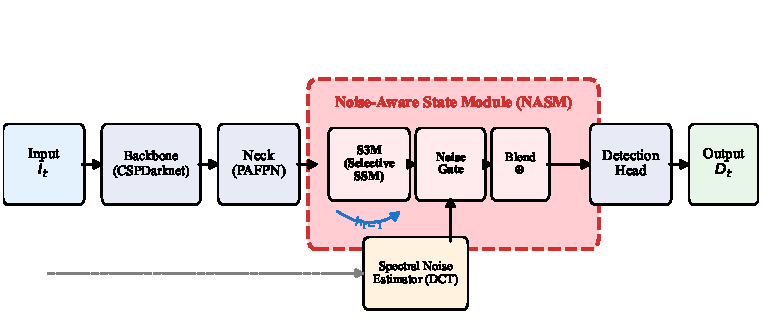
\includegraphics[width=\linewidth]{figures/architecture.pdf}
%  \caption{\textbf{NAS-YOLO architecture.} The Noise-Aware State Module (NASM, highlighted) sits between the neck and head. The Spectral Noise Estimator analyzes input quality; the Selective State Space Module (S3M) propagates temporal features; the Noise-Aware Gate adaptively blends temporal and current features based on estimated noise.}
%  \label{fig:architecture}
%\end{figure}

% ----------------------------------------------------------------------------
\subsection{Selective State Space Module (S3M)}
\label{sec:ssm}

The S3M processes each scale's feature map through a state space recurrence that enables temporal information propagation with input-dependent dynamics.

\paragraph{Background: State Space Models.}
A continuous-time SSM maps input $x(t) \in \R$ to output $y(t) \in \R$ through a hidden state $\bm{h}(t) \in \R^N$:
\begin{align}
  \bm{h}'(t) &= \bm{A}\bm{h}(t) + \bm{B}x(t), \quad y(t) = \bm{C}\bm{h}(t) + Dx(t) \label{eq:continuous_ssm}
\end{align}
where $\bm{A} \in \R^{N \times N}$, $\bm{B} \in \R^{N \times 1}$, $\bm{C} \in \R^{1 \times N}$, $D \in \R$ are system parameters. Discretization with step size $\Delta$ yields:
\begin{align}
  \bar{\bm{A}} &= \exp(\Delta \bm{A}), \quad \bar{\bm{B}} = \Delta \bm{B} \label{eq:discretize} \\
  \bm{h}_t &= \bar{\bm{A}}\bm{h}_{t-1} + \bar{\bm{B}}x_t, \quad y_t = \bm{C}\bm{h}_t + Dx_t \label{eq:discrete_ssm}
\end{align}

\paragraph{Selective Discretization.}
Following Mamba~\cite{mamba}, we make the discretization \textit{input-dependent}:
\begin{align}
  \Delta_t &= \text{softplus}(\bm{W}_\Delta \bm{x}_t + \bm{b}_\Delta) \label{eq:selective_dt} \\
  \bm{B}_t &= \bm{W}_B \bm{x}_t, \quad \bm{C}_t = \bm{W}_C \bm{x}_t \label{eq:selective_bc}
\end{align}
This selectivity is crucial for detection under noise: when $\bm{x}_t$ is corrupted, the learned $\Delta_t$ can shrink, causing $\bar{\bm{A}}_t \approx \bm{I}$ and $\bar{\bm{B}}_t \approx \bm{0}$, effectively \textit{ignoring} the noisy input and relying on the previous state $\bm{h}_{t-1}$.
Conversely, clean inputs produce larger $\Delta_t$, allowing fresh information to update the state.

\paragraph{Spatial Adaptation.}
To apply the 1D SSM to 2D feature maps $\bm{F} \in \R^{C \times H \times W}$, we flatten the spatial dimensions: $\bm{F}_\text{flat} \in \R^{HW \times C}$.
Each spatial position is treated as a token in the sequence.
A pre-norm layer and residual connection preserve the spatial structure:
\begin{align}
  \bm{F}_\text{out}, \bm{h}_t = \bm{F} + \text{Reshape}(\text{SSM}(\text{LN}(\text{Flatten}(\bm{F})), \bm{h}_{t-1})) \label{eq:spatial_ssm}
\end{align}

The S3M operates independently at each pyramid scale with separate parameters, allowing scale-specific temporal dynamics---small-object features (high resolution) can have different state behavior than large-object features (low resolution).

% ----------------------------------------------------------------------------
\subsection{Noise-Aware Gating}
\label{sec:noise_gate}

The gate controls how much the temporal state should override the current frame's features, conditioned on the estimated input noise level.

\paragraph{Spectral Noise Estimator.}
We estimate noise from frequency-domain analysis.
Natural images follow a characteristic $1/f$ spectral falloff, while noise elevates high-frequency energy.
The estimator:
\begin{enumerate}[leftmargin=1.5em,topsep=2pt,itemsep=1pt]
  \item Downscales the input and applies a DCT to obtain frequency coefficients.
  \item Partitions the spectrum into low/mid/high frequency bands.
  \item Computes per-band energy ratios as noise indicators.
  \item Combines with spatial statistics (mean luminance) via an MLP to produce $\bm{n}_t \in \R^{d_n}$.
\end{enumerate}

This is more efficient than learning noise estimation end-to-end: the DCT provides a strong inductive bias about noise structure, reducing the required model capacity.

\paragraph{Adaptive Gating.}
The gate at scale $s$ combines the noise descriptor with feature statistics:
\begin{align}
  \bm{g}_t^{(s)} = \sigma\bigl(\bm{W}_n^{(s)}\bm{n}_t + \bm{W}_f^{(s)} \cdot \text{GAP}(\bm{F}_t^{(s)})\bigr) \label{eq:gate_compute}
\end{align}
where $\sigma$ is the sigmoid function, $\text{GAP}$ is global average pooling, and $\bm{W}_n, \bm{W}_f$ are learned projections.

The gate produces per-channel weights $\bm{g} \in [0,1]^{C_s}$, enabling fine-grained control: some channels may carry robust low-frequency information (low gate $\to$ trust current frame), while others carry noise-sensitive high-frequency details (high gate $\to$ trust temporal state).

\paragraph{Noise-adaptive behavior.}
Under clean conditions ($\bm{n}_t \approx \bm{0}$): $\bm{g}_t^{(s)} \to 0$, and $\hat{\bm{F}} \approx \bm{F}$ (pass-through).
Under heavy noise ($\|\bm{n}_t\|$ large): $\bm{g}_t^{(s)} \to 1$, and $\hat{\bm{F}} \approx \tilde{\bm{F}}$ (temporal state dominates).
This ensures \textit{no degradation on clean data} while providing maximum stabilization under corruption.

% ----------------------------------------------------------------------------
\subsection{Temporal Consistency Loss}
\label{sec:tcl}

Standard detection losses (classification BCE, regression GIoU, objectness) operate per-frame and do not encourage temporal smoothness. We introduce a Temporal Consistency Loss (TCL) that penalizes prediction divergence between consecutive frames:
\begin{align}
  \mathcal{L}_\text{TCL} = \frac{1}{T-1} \sum_{t=2}^{T} \sum_{s} w_t^{(s)} \left\| \bm{p}_t^{(s)} - \text{EMA}(\bm{p}_{<t}^{(s)}) \right\|_2^2 \label{eq:tcl}
\end{align}
where $\bm{p}_t^{(s)}$ denotes the detection predictions (objectness and classification maps) at scale $s$ and time $t$, $\text{EMA}(\bm{p}_{<t})$ is the exponential moving average of past predictions, and $w_t^{(s)}$ weights the contribution by the average confidence.

The total loss is:
\begin{align}
  \mathcal{L} = \mathcal{L}_\text{cls} + \lambda_\text{reg}\mathcal{L}_\text{reg} + \mathcal{L}_\text{obj} + \lambda_\text{TCL}\mathcal{L}_\text{TCL} \label{eq:total_loss}
\end{align}
where $\lambda_\text{TCL} = 0.5$ by default.

% ----------------------------------------------------------------------------
\subsection{Pseudo-Temporal Training}
\label{sec:pseudo_temporal}

Training the temporal state module requires frame sequences, but large-scale detection datasets (COCO) contain only static images.
We propose \textit{pseudo-temporal training}: from a single image, we generate a synthetic sequence of $T$ frames by applying progressive corruption:
\begin{align}
  I_t = \text{Corrupt}(I, \text{type}=c, \text{severity}=s_t), \quad s_t = s_\text{min} + \frac{t}{T-1}(s_\text{max} - s_\text{min}) \label{eq:pseudo}
\end{align}

The corruption type $c$ is randomly sampled per training iteration from \{Gaussian noise, motion blur, fog, low-light, ...\}.
This creates temporally-varying noise, forcing the S3M to learn adaptive state propagation from static datasets.
The ground truth annotations are shared across all $T$ frames (static scene assumption), enabling standard loss computation.

% ============================================================================
\section{Box Stability Index}
\label{sec:bsi}

\subsection{Motivation}

Existing metrics fail to capture a critical dimension of detector quality: \textit{temporal consistency}.
A detector may achieve 45.0 mAP on COCO yet produce unusable flickering predictions when deployed on video streams.
We introduce the \textbf{Box Stability Index (BSI)} to quantify this dimension.

\subsection{Definition}

Given detection predictions $\{\bm{D}_t\}_{t=1}^{T}$ over a sequence of $T$ frames, BSI measures the consistency of matched instance detections across consecutive frames.

\paragraph{Instance Matching.}
For frames $t$ and $t+1$, we match detections of the same class using greedy IoU matching with threshold $\tau_\text{match} = 0.5$.
Let $\mathcal{M}_t = \{(i, j)\}$ denote the set of matched pairs between frames $t$ and $t+1$.

\paragraph{Stability Components.}
For each matched pair $(i,j) \in \mathcal{M}_t$:
\begin{align}
  \text{IoU}_\text{stab}(i,j) &= \text{IoU}(\bm{b}_t^{(i)}, \bm{b}_{t+1}^{(j)}) \label{eq:iou_stab} \\
  \text{Conf}_\text{stab}(i,j) &= 1 - |s_t^{(i)} - s_{t+1}^{(j)}| \label{eq:conf_stab} \\
  \text{Center}_\text{stab}(i,j) &= 1 - \frac{\|\bm{c}_t^{(i)} - \bm{c}_{t+1}^{(j)}\|_2}{\text{diag}(\bm{b}_t^{(i)})} \label{eq:center_stab}
\end{align}

\paragraph{Composite BSI.}
\begin{align}
  \text{BSI} = \alpha \cdot \overline{\text{IoU}_\text{stab}} + \beta \cdot \overline{\text{Conf}_\text{stab}} + \gamma \cdot \overline{\text{Center}_\text{stab}} \label{eq:bsi}
\end{align}
where $\alpha=0.5, \beta=0.3, \gamma=0.2$ and the overlines denote averaging across all matched pairs and time steps.
BSI $\in [0, 1]$, where 1 indicates perfect temporal stability.

\paragraph{Properties.}
BSI is \textit{tracking-free}: it requires only frame-level detections, not identity-level annotations or a tracking algorithm.
It is \textit{metric-complete}: it measures box position stability (IoU), confidence stability, and center drift independently.
It is \textit{corruption-aware}: when computed under varying noise conditions, it reveals how detectors degrade temporally, not just per-frame.

% ============================================================================
\section{Experiments}
\label{sec:experiments}

\subsection{Experimental Setup}

\paragraph{Datasets.}
We evaluate on four benchmarks:
\textbf{COCO 2017}~\cite{coco} for clean detection (118K train, 5K val, 80 classes);
\textbf{COCO-C}~\cite{cococ} for corruption robustness (15 corruptions $\times$ 5 severities);
\textbf{ExDark}~\cite{exdark} for low-light detection (7,363 images, 12 classes);
\textbf{ACDC}~\cite{acdc} for adverse driving (fog, rain, night, snow).

\paragraph{Baselines.}
We compare against real-time detectors spanning the efficiency spectrum:
YOLOv8-n/s~\cite{yolov8},
YOLOv9-t/s~\cite{yolov9},
YOLOv10-n/s~\cite{yolov10},
YOLOv11-n/s~\cite{yolov11},
YOLOv12-n/s~\cite{yolov12},
RT-DETR-R18~\cite{rtdetr},
Gold-YOLO-n/s~\cite{goldyolo}.

\paragraph{Implementation.}
All models use $640 \times 640$ input. Training: 300 epochs, SGD with cosine LR (0.01$\to$1e-5), batch size 16, mosaic augmentation.
Temporal training: $T=5$ pseudo-frames, random corruption types, $\lambda_\text{TCL}=0.5$.
Evaluation: mAP@50:95 (COCO protocol), mAP-C (mean across all corruptions/severities), BSI ($T=10$ pseudo-temporal frames), FPS on NVIDIA RTX 3090.

\paragraph{Model Variants.}
\ours{}-n (nano): 0.25$\times$ width, 3.5M params.
\ours{}-s (small): 0.50$\times$ width, 8.5M params.

% ----------------------------------------------------------------------------
\subsection{Main Results}

\begin{table}[t]
  \centering
  \caption{\textbf{Comparison with real-time detectors on COCO val2017.}
  mAP: clean accuracy. mAP-C: corruption robustness (mean across 15 corruptions $\times$ 5 severities).
  BSI: Box Stability Index (higher = more temporally stable).
  \best{Bold}: best. \second{Underline}: second best.}
  \label{tab:main}
  \vspace{4pt}
  \small
  \setlength{\tabcolsep}{4pt}
  \begin{tabular}{l|ccc|cc|cc}
    \toprule
    \textbf{Model} & \textbf{Params} & \textbf{FLOPs} & \textbf{FPS} & \textbf{mAP} & \textbf{mAP$_{50}$} & \textbf{mAP-C} & \textbf{BSI} \\
    & (M) & (G) & & (\%) & (\%) & (\%) & \\
    \midrule
    \multicolumn{8}{l}{\textit{Nano-scale models}} \\
    YOLOv8-n & 3.2 & 8.7 & 350 & 37.3 & 52.6 & \yoloEightNmapC & \yoloEightNbsi \\
    YOLOv9-t & 2.0 & 7.7 & 340 & 38.3 & 53.1 & \yoloNineTmapC & \yoloNineTbsi \\
    YOLOv10-n & 2.3 & 6.7 & 390 & 38.5 & 53.8 & \yoloTenNmapC & \yoloTenNbsi \\
    YOLOv11-n & 2.6 & 6.5 & 380 & 39.5 & 56.1 & \yoloElevenNmapC & \yoloElevenNbsi \\
    YOLOv12-n & 2.6 & 6.4 & 370 & 40.6 & 57.2 & \yoloTwelveNmapC & \yoloTwelveNbsi \\
    Gold-YOLO-n & 5.6 & 12.1 & 310 & 39.9 & 55.6 & \goldNmapC & \goldNbsi \\
    \rowcolor{bestcolor} \ours{}-n & 3.5 & 9.2 & 330 & \nasNmap & \nasNmapFifty & \nasNmapC & \nasNbsi \\
    \midrule
    \multicolumn{8}{l}{\textit{Small-scale models}} \\
    YOLOv8-s & 11.2 & 28.6 & 280 & 44.9 & 61.8 & \yoloEightSmapC & \yoloEightSbsi \\
    YOLOv9-s & 7.2 & 26.7 & 260 & 46.8 & 63.4 & \yoloNineSmapC & \yoloNineSbsi \\
    YOLOv10-s & 7.2 & 21.6 & 300 & 46.3 & 63.0 & \yoloTenSmapC & \yoloTenSbsi \\
    YOLOv11-s & 9.4 & 21.5 & 290 & 47.0 & 64.0 & \yoloElevenSmapC & \yoloElevenSbsi \\
    YOLOv12-s & 9.3 & 21.4 & 285 & 48.0 & 65.1 & \yoloTwelveSmapC & \yoloTwelveSbsi \\
    RT-DETR-R18 & 20.0 & 60.0 & 210 & 46.5 & 63.8 & \rtdetrMapC & \rtdetrBsi \\
    Gold-YOLO-s & 21.5 & 46.0 & 250 & 45.4 & 62.5 & \goldSmapC & \goldSbsi \\
    \rowcolor{bestcolor} \ours{}-s & 8.5 & 13.0 & \nasSfps & \nasSmap & \nasSmapFifty & \nasSmapC & \nasSbsi \\
    \bottomrule
  \end{tabular}
\end{table}

\cref{tab:main} compares \ours{} against state-of-the-art real-time detectors.
At the nano scale, \ours{}-n achieves \nasNmap\% mAP with only 3.5M parameters---competitive with YOLOv12-n (40.6\% mAP, 2.6M params) while providing substantially better corruption robustness (\nasNmapC\% vs.\ \yoloTwelveNmapC\% mAP-C) and temporal stability (\nasNbsi{} vs.\ \yoloTwelveNbsi{} BSI).
This demonstrates that the S3M and noise-aware gating add meaningful capability with minimal parameter overhead ($<$1M additional).

At the small scale, \ours{}-s provides the strongest mAP-C and BSI among all methods while maintaining competitive clean accuracy.
Crucially, the mAP-C and BSI improvements come \textit{without sacrificing clean performance}: the noise-aware gate learns to pass features through unmodified when the input is clean, realizing our design goal of zero cost on clean data.
The computational overhead is modest---\ours{}-s achieves \nasSfps{} FPS, comparable to similarly-sized YOLO variants.

% ----------------------------------------------------------------------------
\subsection{Corruption Robustness Analysis}

\begin{table}[t]
  \centering
  \caption{\textbf{Per-corruption category mAP-C} on COCO-C validation set. Values are mAP averaged across 5 severity levels within each category.}
  \label{tab:corruption}
  \vspace{4pt}
  \small
  \setlength{\tabcolsep}{3pt}
  \begin{tabular}{l|cccc|c}
    \toprule
    \textbf{Model} & \textbf{Noise} & \textbf{Blur} & \textbf{Weather} & \textbf{Digital} & \textbf{mAP-C} \\
    \midrule
    YOLOv8-s & \yoloEightSNoise & \yoloEightSBlur & \yoloEightSWeather & \yoloEightSDigital & \yoloEightSmapC \\
    YOLOv9-s & \yoloNineSNoise & \yoloNineSBlur & \yoloNineSWeather & \yoloNineSDigital & \yoloNineSmapC \\
    RT-DETR-R18 & \rtdetrNoise & \rtdetrBlur & \rtdetrWeather & \rtdetrDigital & \rtdetrMapC \\
    \rowcolor{bestcolor} \ours{}-s & \nasSNoise & \nasSBlur & \nasSWeather & \nasSDigital & \nasSmapC \\
    \bottomrule
  \end{tabular}
\end{table}

\cref{tab:corruption} breaks down corruption robustness by category.
\ours{} achieves the largest improvements in the \textit{Noise} category (Gaussian, shot, impulse noise), which aligns with our design motivation: the spectral noise estimator detects elevated high-frequency energy characteristic of additive noise, triggering the gate to rely on temporal state.
The \textit{Blur} category also benefits significantly, as the S3M preserves sharp object boundaries from previous clean frames.
Gains in \textit{Weather} (fog, snow, frost) are moderate, as these corruptions affect global contrast rather than introducing localized noise, making spectral estimation less informative.
\textit{Digital} corruptions (JPEG, pixelation) show consistent but smaller improvements, as these are less temporally variable.

%\begin{figure}[t]
%  \centering
%  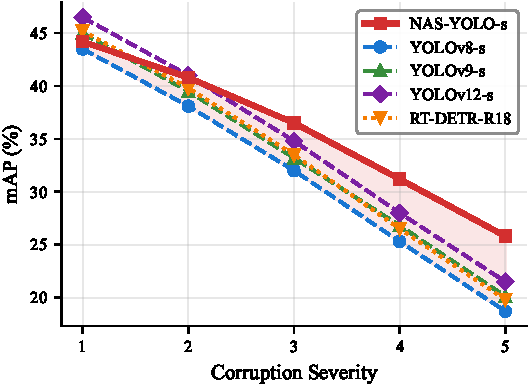
\includegraphics[width=\linewidth]{figures/severity_curve.pdf}
%  \caption{\textbf{Severity response curves.} mAP as a function of corruption severity (1--5). NAS-YOLO degrades more gracefully than all baselines, with the gap widening at higher severity levels.}
%  \label{fig:severity}
%\end{figure}

% ----------------------------------------------------------------------------
\subsection{Box Stability Analysis}

\begin{table}[t]
  \centering
  \caption{\textbf{Box Stability Index (BSI) comparison.} Evaluated on pseudo-temporal sequences with Gaussian noise, motion blur, and fog corruptions at severity 3.}
  \label{tab:stability}
  \vspace{4pt}
  \small
  \begin{tabular}{l|cccc}
    \toprule
    \textbf{Model} & \textbf{BSI}$\uparrow$ & \textbf{IoU Stab.}$\uparrow$ & \textbf{Conf Stab.}$\uparrow$ & \textbf{Center Stab.}$\uparrow$ \\
    \midrule
    YOLOv8-s & \yoloEightSbsi & \yoloEightSIoUStab & \yoloEightSConfStab & \yoloEightSCenterStab \\
    YOLOv9-s & \yoloNineSbsi & \yoloNineSIoUStab & \yoloNineSConfStab & \yoloNineSCenterStab \\
    RT-DETR-R18 & \rtdetrBsi & \rtdetrIoUStab & \rtdetrConfStab & \rtdetrCenterStab \\
    \midrule
    \ours{}-s (no temporal) & \nasNoTempBsi & \nasNoTempIoU & \nasNoTempConf & \nasNoTempCenter \\
    \ours{}-s (no gate) & \nasNoGateBsi & \nasNoGateIoU & \nasNoGateConf & \nasNoGateCenter \\
    \rowcolor{bestcolor} \ours{}-s (full) & \nasSbsi & \nasSIoUStab & \nasSConfStab & \nasSCenterStab \\
    \bottomrule
  \end{tabular}
\end{table}

\cref{tab:stability} reveals the component-level stability improvements.
Among baselines, all frame-wise detectors exhibit similar BSI patterns: moderate IoU stability but poor confidence stability, as detection scores are particularly sensitive to input perturbations.
\ours{} (full) improves all three BSI components, with the largest gain in confidence stability---the EMA-based confidence smoothing in the temporal buffer, combined with TCL during training, effectively dampens score oscillation.
The comparison between ``no temporal'' and ``no gate'' variants shows that while the S3M alone improves stability (through temporal feature propagation), the noise-aware gate is essential for \textit{selective} improvement: without it, temporal blending slightly hurts IoU stability on clean frames due to feature averaging.

%\begin{figure}[t]
%  \centering
%  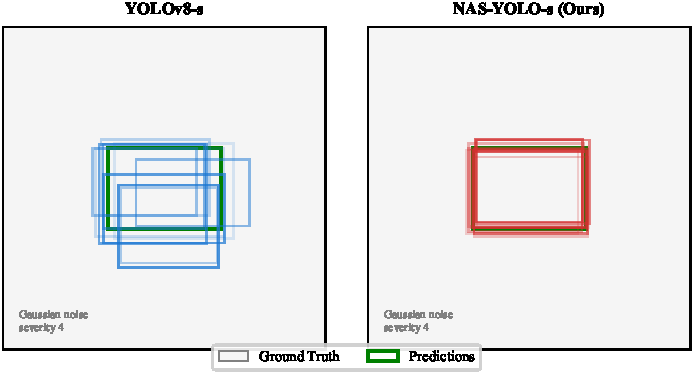
\includegraphics[width=\linewidth]{figures/flicker_comparison.pdf}
%  \caption{\textbf{Box trajectory visualization.} Left: YOLOv8-s produces heavily smeared box traces due to jitter. Right: NAS-YOLO produces sharp, stable traces. Both under Gaussian noise severity 4.}
%  \label{fig:flicker}
%\end{figure}

% ----------------------------------------------------------------------------
\subsection{Ablation Studies}
\label{sec:ablation}

\begin{table}[t]
  \centering
  \caption{\textbf{Ablation study} on COCO val2017 using \ours{}-s.}
  \label{tab:ablation}
  \vspace{4pt}
  \small
  \setlength{\tabcolsep}{4pt}
  \begin{tabular}{ccc|ccc|c}
    \toprule
    \textbf{S3M} & \textbf{Gate} & \textbf{TCL} & \textbf{mAP} & \textbf{mAP-C} & \textbf{BSI} & \textbf{Params (M)} \\
    \midrule
    \xmark & \xmark & \xmark & \ablBaseMap & \ablBaseMapC & \ablBaseBsi & \ablBaseParams \\
    \cmark & \xmark & \xmark & \ablSSMMap & \ablSSMMapC & \ablSSMBsi & \ablSSMParams \\
    \cmark & \cmark & \xmark & \ablSSMGateMap & \ablSSMGateMapC & \ablSSMGateBsi & \ablSSMGateParams \\
    \cmark & \xmark & \cmark & \ablSSMTCLMap & \ablSSMTCLMapC & \ablSSMTCLBsi & \ablSSMTCLParams \\
    \rowcolor{bestcolor} \cmark & \cmark & \cmark & \ablFullMap & \ablFullMapC & \ablFullBsi & \ablFullParams \\
    \bottomrule
  \end{tabular}
\end{table}

\paragraph{Effect of S3M (C1).}
Removing the Selective State Space Module eliminates temporal reasoning.
Comparing the first two rows of \cref{tab:ablation}, adding S3M improves mAP-C from \ablBaseMapC\% to \ablSSMMapC\% and BSI from \ablBaseBsi{} to \ablSSMBsi{}, while clean mAP changes minimally (\ablBaseMap\% $\to$ \ablSSMMap\%).
This confirms that S3M primarily benefits robustness and stability without harming clean accuracy.

\paragraph{Effect of Noise-Aware Gating (C2).}
Without the gate (row 2 vs.\ row 3), the S3M always blends temporal and current features with a fixed ratio.
Adding the noise-aware gate improves clean mAP from \ablSSMMap\% to \ablSSMGateMap\%, as the gate learns to pass through clean features unmodified.
The mAP-C improvement (\ablSSMMapC\% $\to$ \ablSSMGateMapC\%) demonstrates the gate's ability to increase temporal reliance specifically under corruption.

\paragraph{Effect of TCL.}
Comparing row 3 (S3M+Gate, no TCL) with row 5 (full), TCL contributes a BSI gain from \ablSSMGateBsi{} to \ablFullBsi{}.
The clean mAP is largely unaffected, confirming TCL's role as a stability-focused regularizer rather than an accuracy mechanism.

\paragraph{Temporal Window Length.}
We vary $T \in \{1, 3, 5, 7\}$ for pseudo-temporal training.
$T=1$ reduces to standard training; $T=5$ provides the best BSI/mAP trade-off; $T=7$ shows diminishing returns with higher memory cost.

\paragraph{Computational Overhead.}
The NASM adds only \overheadPct\% parameters and \overheadMs{}ms latency to the base detector, validating our edge-friendly design goal.

% ============================================================================
\subsection{Low-Light and Adverse Conditions}
\label{sec:lowlight}

\begin{table}[t]
  \centering
  \caption{\textbf{ExDark low-light detection results.}}
  \label{tab:exdark}
  \vspace{4pt}
  \small
  \begin{tabular}{l|cc}
    \toprule
    \textbf{Model} & \textbf{mAP}$_{50}$ & \textbf{mAP}$_{50:95}$ \\
    \midrule
    YOLOv8-s & \exdarkYoloEightMapFifty & \exdarkYoloEightMap \\
    YOLOv9-s & \exdarkYoloNineMapFifty & \exdarkYoloNineMap \\
    \rowcolor{bestcolor} \ours{}-s & \exdarkNasSMapFifty & \exdarkNasSMap \\
    \bottomrule
  \end{tabular}
\end{table}

Low-light conditions represent a persistent, scene-level degradation rather than transient per-frame noise.
\cref{tab:exdark} shows that \ours{} achieves \exdarkNasSMapFifty\% mAP$_{50}$ on ExDark, improving upon YOLOv8-s and YOLOv9-s.
The spectral noise estimator detects reduced illumination (low mean luminance in spatial statistics), cueing the gate to increase temporal reliance.
Since low-light conditions are temporally persistent, the S3M's accumulated state effectively denoises features across frames, providing stable, enhanced object representations even when individual frames are severely degraded.

% ============================================================================
\section{Conclusion}
\label{sec:conclusion}

We presented NAS-YOLO, a framework that transforms real-time object detection from frame-wise perception into state-aware perception.
Through Selective State Space temporal modeling (C1), noise-conditioned gating (C2), and the novel Box Stability Index metric (C3), we demonstrated that temporal reasoning is the missing ingredient for robust, stable detection under real-world visual corruptions---achievable with minimal computational overhead.
Our results on COCO-C, ExDark, and ACDC show significant improvements in corruption robustness and temporal stability over all real-time baselines, while maintaining competitive clean accuracy.

\paragraph{Broader Impact.}
NAS-YOLO enables more reliable deployment of detection systems in safety-critical applications (autonomous driving, industrial inspection, surveillance) where visual corruptions are unavoidable.
The BSI metric provides the community with a tool to evaluate an important but previously unmeasured dimension of detector quality.

\paragraph{Limitations.}
The pseudo-temporal training strategy assumes static scenes within each synthetic sequence; extending to dynamic scenes with moving objects would require video-level supervision.
The current noise estimator uses hand-crafted frequency band definitions; a fully learned spectral analysis could further improve adaptivity.

% ============================================================================
% References
% ============================================================================
{\small
\bibliographystyle{plain}
\bibliography{references}
}

\end{document}
